In this section, we describe the main methodological contribution of this article, the development of a three-step methodology for assessing managerial preferences on the attributes of team members. Our method consists of the following components, which are described in detail below:
\begin{enumerate}
\item Definition of the evaluation dimensions according to the literature,
\item Confirming these findings with the managerial point of view, and
\item Elicitation of the managerial evaluating model of the team members based on the defined criteria.
\end{enumerate}
The method is a classic one: first an open discussion with the DMs about what matters to them, then their evaluation of the formalization of the criteria proposed by the literature, and finally elicitation of their priorities. Here we describe the process more generally, while in Section~\ref{sec:results} we show an example application for the domain of FLOSS development.

\subsection{Defining the dimensions for evaluating team members}

In order for a DM to assess a team member as good or bad, it is first necessary to identify the characteristics which are used in that evaluation. While the literature does not specifically address the question of the alignment of the team member's characteristics with the team leader's expectations, it does provide a general description of the criteria. In Section~\ref{sec:related} we detailed five psycho-sociological dimensions which can be universally applied to teaming situations. These characteristics are meant to be used in conjunction with the technical attributes, which vary by domain. 


In the first step, a number of DMs with experience in the domain are 
asked which attributes they consider relevant for identifying a team member's
value to the group.  We make use of interviews in order to gain an understanding of the DM and
the language and context of the decision \citep{Myers97}.


%%%% Modif here %%%%
After giving their responses, DMs are then supplied with a list of characteristics
the researchers have gleaned from the literature and asked to indicate how
relevant these characteristics are (in the case of this paper, the characteristics are introduced in Section~\ref{sec:related} and detailed in Section~\ref{sec:results}). Finally, they are asked if they want to
add any characteristics to their initial list. This allows the participant
to first consider the question without being primed, then to evaluate the
criteria from literature, and finally to reflect on the initial thoughts.

%%% End of modif %%%%

The interview responses are compared to the initial list derived from the
literature. Where the DMs described existing criteria using different terms,
the names or descriptions of the criteria are updated to reflect the 
language of the participants. If any new criteria are identified, this
may warrant additional study to understand why it was not previously
described in the literature. When a particular criteria is not valued by
any participants, the criteria could be dropped to reduce the number of
dimensions to be considered.

As previously stated, this part of the methodology is quite mainstream. The psycho-social components are applicable to any teaming analysis, and while the technical ones are more specific, the process of creating the list of attributes is familiar to researchers. The specific elements of our methodology begin in the second step, with preparing the complete list of criteria for MCDA.

\subsection{Selecting the criteria for the MCDA analysis}

Selecting the criteria for an MCDA process requires reducing the options to a manageable level.  According to \cite{mil56}, there are limits to human capacity for processing information, which explains why the maximum number of aspects which can be simultaneously considered is around seven, plus or minus two. From our literature review and initial interviews, we were able to narrow the dimensions to ten by excluding factors which were not valued by any DM.

In order to extract the subset of dimensions relevant for each DM, we asked them to rate each dimension based on their perception of its importance with one of five levels, ranging from {\em very important} to {\em not important at all}. We then included all criteria they ranked as very important or important. It is worth noting that in other types of analysis of preferences, such as Q-methodology, the standard is to incorporate those factors which can explain at least 50\% of the sample variance \citep{wingreen:2005:assessing}. If we considered each factor equally important to the DM, incorporating five dimensions would already capture half of the variance. However, based on the DM's rankings, it was certain that by dropping the less important factors we were reducing the demands on the DM without significant loss of detail.

\subsection{Inferring the DM's preferences}

In Section~\ref{sec:MCDA}, we explained why we advocated using the MR-Sort technique to model the DM preferences. To infer the parameters of such an MR-Sort preference model, the following protocol, illustrated in Figure~\ref{fig:methodology1}, is applied. 

\begin{figure}
\centering
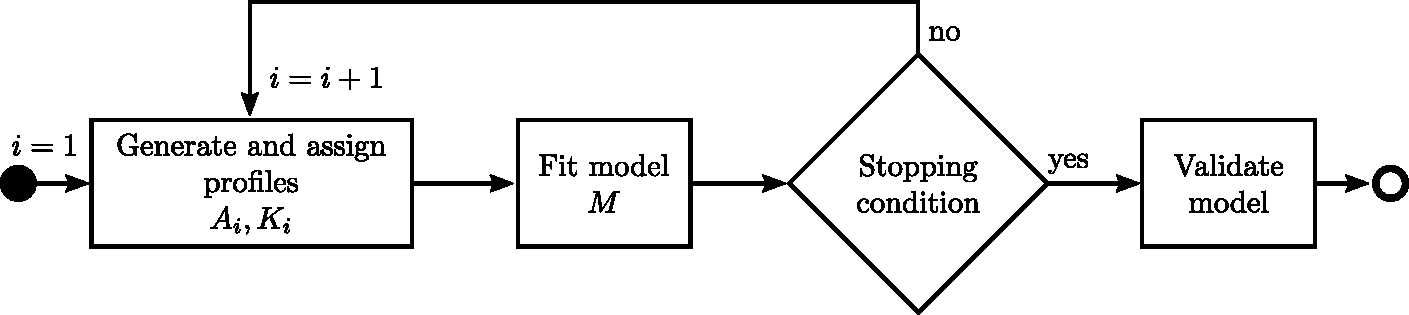
\includegraphics[scale = 0.7]{fig/expdesign1}
\caption{Protocol for inferring the parameters of an MR-Sort model}\label{fig:methodology1}
\end{figure}

The protocol consists of a series of iterations, denoted using the variable $i$.  It begins by randomly generating an initial set of member profiles, denoted with $A_i$, and having the DM assign them to categories, which are denoted with $K_i$. Especially in the initial iterations, conducting this step
interactively provides greater support for the results, as the
articulated perspective in the interview can be compared with the
model derived from the assignment examples:
a form of mixed methods triangulation \citep{Myers97}. 

The second step consists in fitting a model based on these assignments, followed by checking whether a stopping condition is met. 
The stopping condition might be based on subjective factors linked to the willingness of the DM to proceed further, or on factors linked to the fit and convergence of the model. 
If such a stopping condition is met, one proceeds to validating the model, otherwise a new iteration starts by generating an additional set of profiles. Starting with the second iteration, these profiles are generated based on the model $M$.

The second step of fitting a model over $A_j$ and $K_j$, $\forall j \in 1..i$, consists of several additional iterations which are illustrated in Figure~\ref{fig:methodology2}.

\begin{figure}
\centering
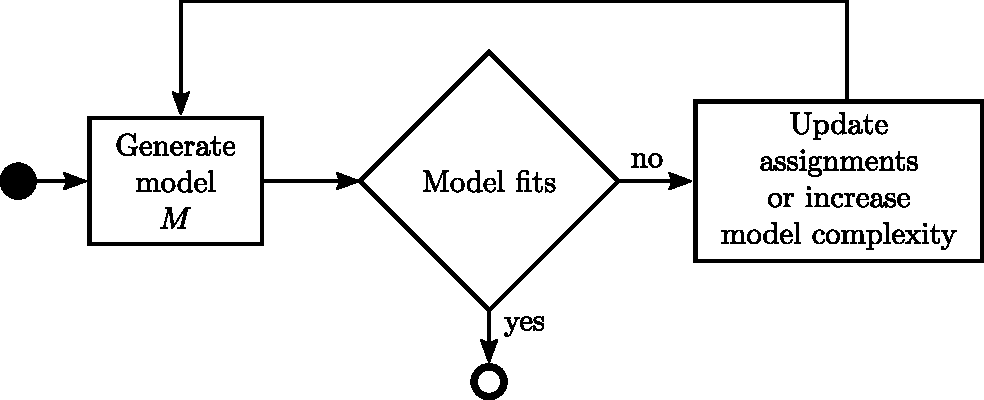
\includegraphics[scale = 0.7]{fig/expdesign2}
\caption{Protocol for fitting an MR-Sort model over a set of assignment examples}\label{fig:methodology2}
\end{figure}

Figure~\ref{fig:methodology1} begins with generating a model from all of the assignment examples from the previous iterations of the protocol. The first iteration starts with a simple MR-Sort model with no vetoes and no dictators, whereas the subsequent iterations start with the type of model previously generated. Fitting is described in Figure~\ref{fig:methodology2}. If the model fits perfectly with the assignment examples, the protocol reverts to the main sequence of steps described in Figure~\ref{fig:methodology1}. If the model does not fit, either the assignment examples are updated or the complexity of the model is increased to represent the assignments. Updating the assignment examples involves generating minimal subsets of profiles and their corresponding alternative assignments, which are then presented to the DM for validation. In increasing the complexity of the model, the {\em principle of parsimony} is applied, in that the simplest explanation is chosen, and complexity is only increased when it is necessary to fit the data. If the initial model which currently does not fit the assignments is, for example, an MR-Sort with a simple majority rule, the closest more complex model would be MR-Sort models with vetoes or dictators, followed by variants weakened by a dictator or a veto, and finally MR-Sort models with both vetoes and dictators. In cases where two equally complex models equally describe most of the assignment examples, one is chosen randomly. Once a fit is obtained, a new iteration of the initial protocol is started.

The next section illustrates with an example the three different stages of the methodology, demonstrating concretely how they can be implemented, and showing what kind of results this method produces.
